Im Folgenden werden bei der Nennung von \glqq Wellen\grqq{} immer Transversalwellen gemeint, wenn es keine weitere Anmerkung gibt.  


\subsection[Ausbreitung in Elementarwellen]{Ausbreitung in Elementarwellen (Huygens'sches Prinzip)} \label{subsec:ausbreitung}

Das Huygens'sche Prinzip macht eine wichtige Aussage zur Ausbreitung von Wellen:

\glqq Jedes Teilchen (Oszillator), das von einer Wellenfront erfasst wird, löst von sich aus eine zirkulare Welle nach allen Seiten aus.\grqq{} Die eigentlich sichtbare Wellenfront ist nach Huygens eine Einhüllende aller \glqq Elementarwellen\grqq . Dadurch ist es Wellen unter anderem möglich, in den geometrischen Schattenraum zu propagieren (Siehe: \referenz{sec:interferenz_spalt}).


\subsection{Reflexion}  \label{subsec:Reflexion}

	\subsubsection{Fixiertes Ende}
	
	Wenn eine Welle von einem fixierten Ende (eingespannt) reflektiert wird, dann gibt es einen Phasensprung von $180 \degree$ oder $\pi$, bzw $\frac{\lambda}{2}$.
	
	\subsubsection{Loses Ende}
	
	Trifft eine Welle auf ein loses Ende, dann wird sie ohne Phasensprung reflektiert.



\subsection{Überlagerung} \label{subsec:ueberlagerung}

Wenn sich Wellen in einem räumlichen Punkt treffen, dann überlagern sie sich und bilden eine summierte Schwingung. Wenn also ein Wellenberg auf einen Wellenberg trifft, addieren sich beide Wellen und das Teilchen in welchem sich die Wellen überlagern wird höher ausgelenkt, als wenn nur eine Welle das Teilchen auslenkt.

Sollte auf einen Wellenberg ein Wellental treffen, wird ebenfalls addiert, wobei dann das Resultat eine kleinere Amplitude ist.

Nachdem sich die Wellen in diesem Punkt überlagert haben, laufen beide weiter ohne die andere zu beeinflussen, so als hätte es die Überlagerung nie gegeben.


\subsection{Interferenzen} \label{subsec:interferenz}

Wenn sich Wellen, die eine identische Wellenlänge besitzen, in einem Punkt überlagern, dann kommt es zu zeitlich stabilen Interferenzen, weil nun die beiden Wellen aus den unterschiedlichen Richtungen mit der selben Frequenz Wellenberge und Wellentäler \glqq nachliefern\grqq{} und damit die Interferenz aufrecht erhalten bleibt.

Der Gangunterschied der beiden Wellen ist $\delta$: die Differenz der Strecken vom jeweiligen Ursprungspunkt (zwei Punkte, in denen die Wellen nicht phasenverschoben sind, also zum selben Zeitpunkt Maxima oder Minima, etc. auftreten) zu dem in Frage stehenden Überlagerungspunkt. Siehe Abbildung \ref{fig:gangunterschied}\endnote{\glqq Interferenzbedingungen\grqq{} von Till Blaha - Eigenes Werk. Lizenziert unter Gemeinfrei.}.

Für die beiden extremen Arten der Interferenz (konstruktiv und destruktiv) muss für $\delta$ eine bestimmte Interferenzbedingungen erfüllt sein.
 
\begin{figure}[!h]
		\centering
		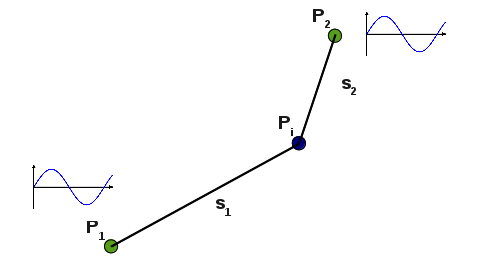
\includegraphics[width=0.9\textwidth]{Interferenz}
		\begin{comment} gnuplot './plot_noticszero.p'
set output 'plot_inteferenzhelper.png'
plot sin(x) ls 3
		\end{comment}
		\caption{$P_1$ und $P_2$ sind die Ursprungspunkte in denen Phasengleichheit herrscht. Die Differenz der Strecken $s_1$ und $s_2$ ist der Gangunterschied $\delta$. Die beiden Elongation-Zeit-Diagramme sollen die zeitliche Phasengleichheit in den beiden Ausgangspunkten zeigen.}
		\label{fig:gangunterschied}
\end{figure}

	\subsubsection{Konstruktive Interferenz}
	
	Bei der konstruktiven Interferenz ist die resultierende Amplitude genau die Addition der Amplituden der Ausgangswellen; das doppelte einer Amplitude, wenn beide Ausgangswellen identische Amplituden besitzen.
	
	Dazu müssen die Wellen im Interferenzpunkt zur selben Zeit Maxima und Minima aufweisen, also muss der Gangunterschied ein ganzzahliges Vielfaches der Wellenlänge sein:
	
	\begin{align}	\label{eq:kon_interferenz}
	\begin{split}
		\delta = k \cdot \lambda \quad \text{wobei} \ k \in 0,1,2...
	\end{split}
	\end{align}
	
	\subsubsection{Destruktive Interferenz}
	
	Bei der destruktiven Interferenz ist die resultierende Amplitude 0, wenn man davon ausgeht, dass die einfallenden Wellen die gleiche Amplitude haben
	
	Der Gangunterschied $\delta$ muss daher die Summe eines ganzzahliges Vielfaches Wellenlänge und der halben Wellenlänge sein, sodass sich immer ein Schwingungsberg und Schwingungstal überlagern und auslöschen.
	
	\begin{align}	\label{eq:des_interferenz}
	\begin{split}
		\delta &= k \cdot \lambda - \frac{\lambda}{2} \quad \text{wobei} \ k \in 1,2,3... \\
		\delta &= \lambda \cdot (k - \frac{1}{2}) \quad \text{wobei} \ k \in 1,2,3... 
	\end{split}
	\end{align}
	

\subsection{Stehende Welle}
	
Wenn sich gegenläufige Wellen, das heißt parallel und identisch, aber sich in die entgegengesetzte Richtung ausbreitende Wellen, mit derselben Wellenlänge überlagern, entsteht eine stehende Welle. 

Das heißt, dass es mindestens 2 Punkte auf gibt, in denen sich die Oszillatoren gar nicht bewegen (\glqq stehen\grqq), die sogenannten Knotenpunkte, in welchen destruktive Interferenz herrscht. Gleichzeitig gibt es auch immer mindestens einen Punkt, in welchem konstruktive Interferenz herrscht.
	
Eine stehende Welle kann zum Beispiel ausgelöst werden, wenn bei einer Reflexion am festen Ende die Hälfte der Wellenlänge $\lambda$ ein ganzzahliges Vielfaches der Abstands $l$ der beiden Enden ist. $k$ ist in diesem Fall eine Variable, die nur positive ganze Zahlen annehmen kann:
	
	\begin{align} \label{eq:stehendewelle}
		l = \frac{k \cdot \lambda}{2} \quad wobei \ k \in 1,2,3...
	\end{align}
	
	
\subsubsection{Beispiel}

Wer Gitarre spielt, erlebt, idealisiert, eine stehende Welle mit $k=0$, wenn er eine offene Saite anschlägt. (Abbildung \ref{fig:grundton})

\begin{figure}[!h]
		\centering
		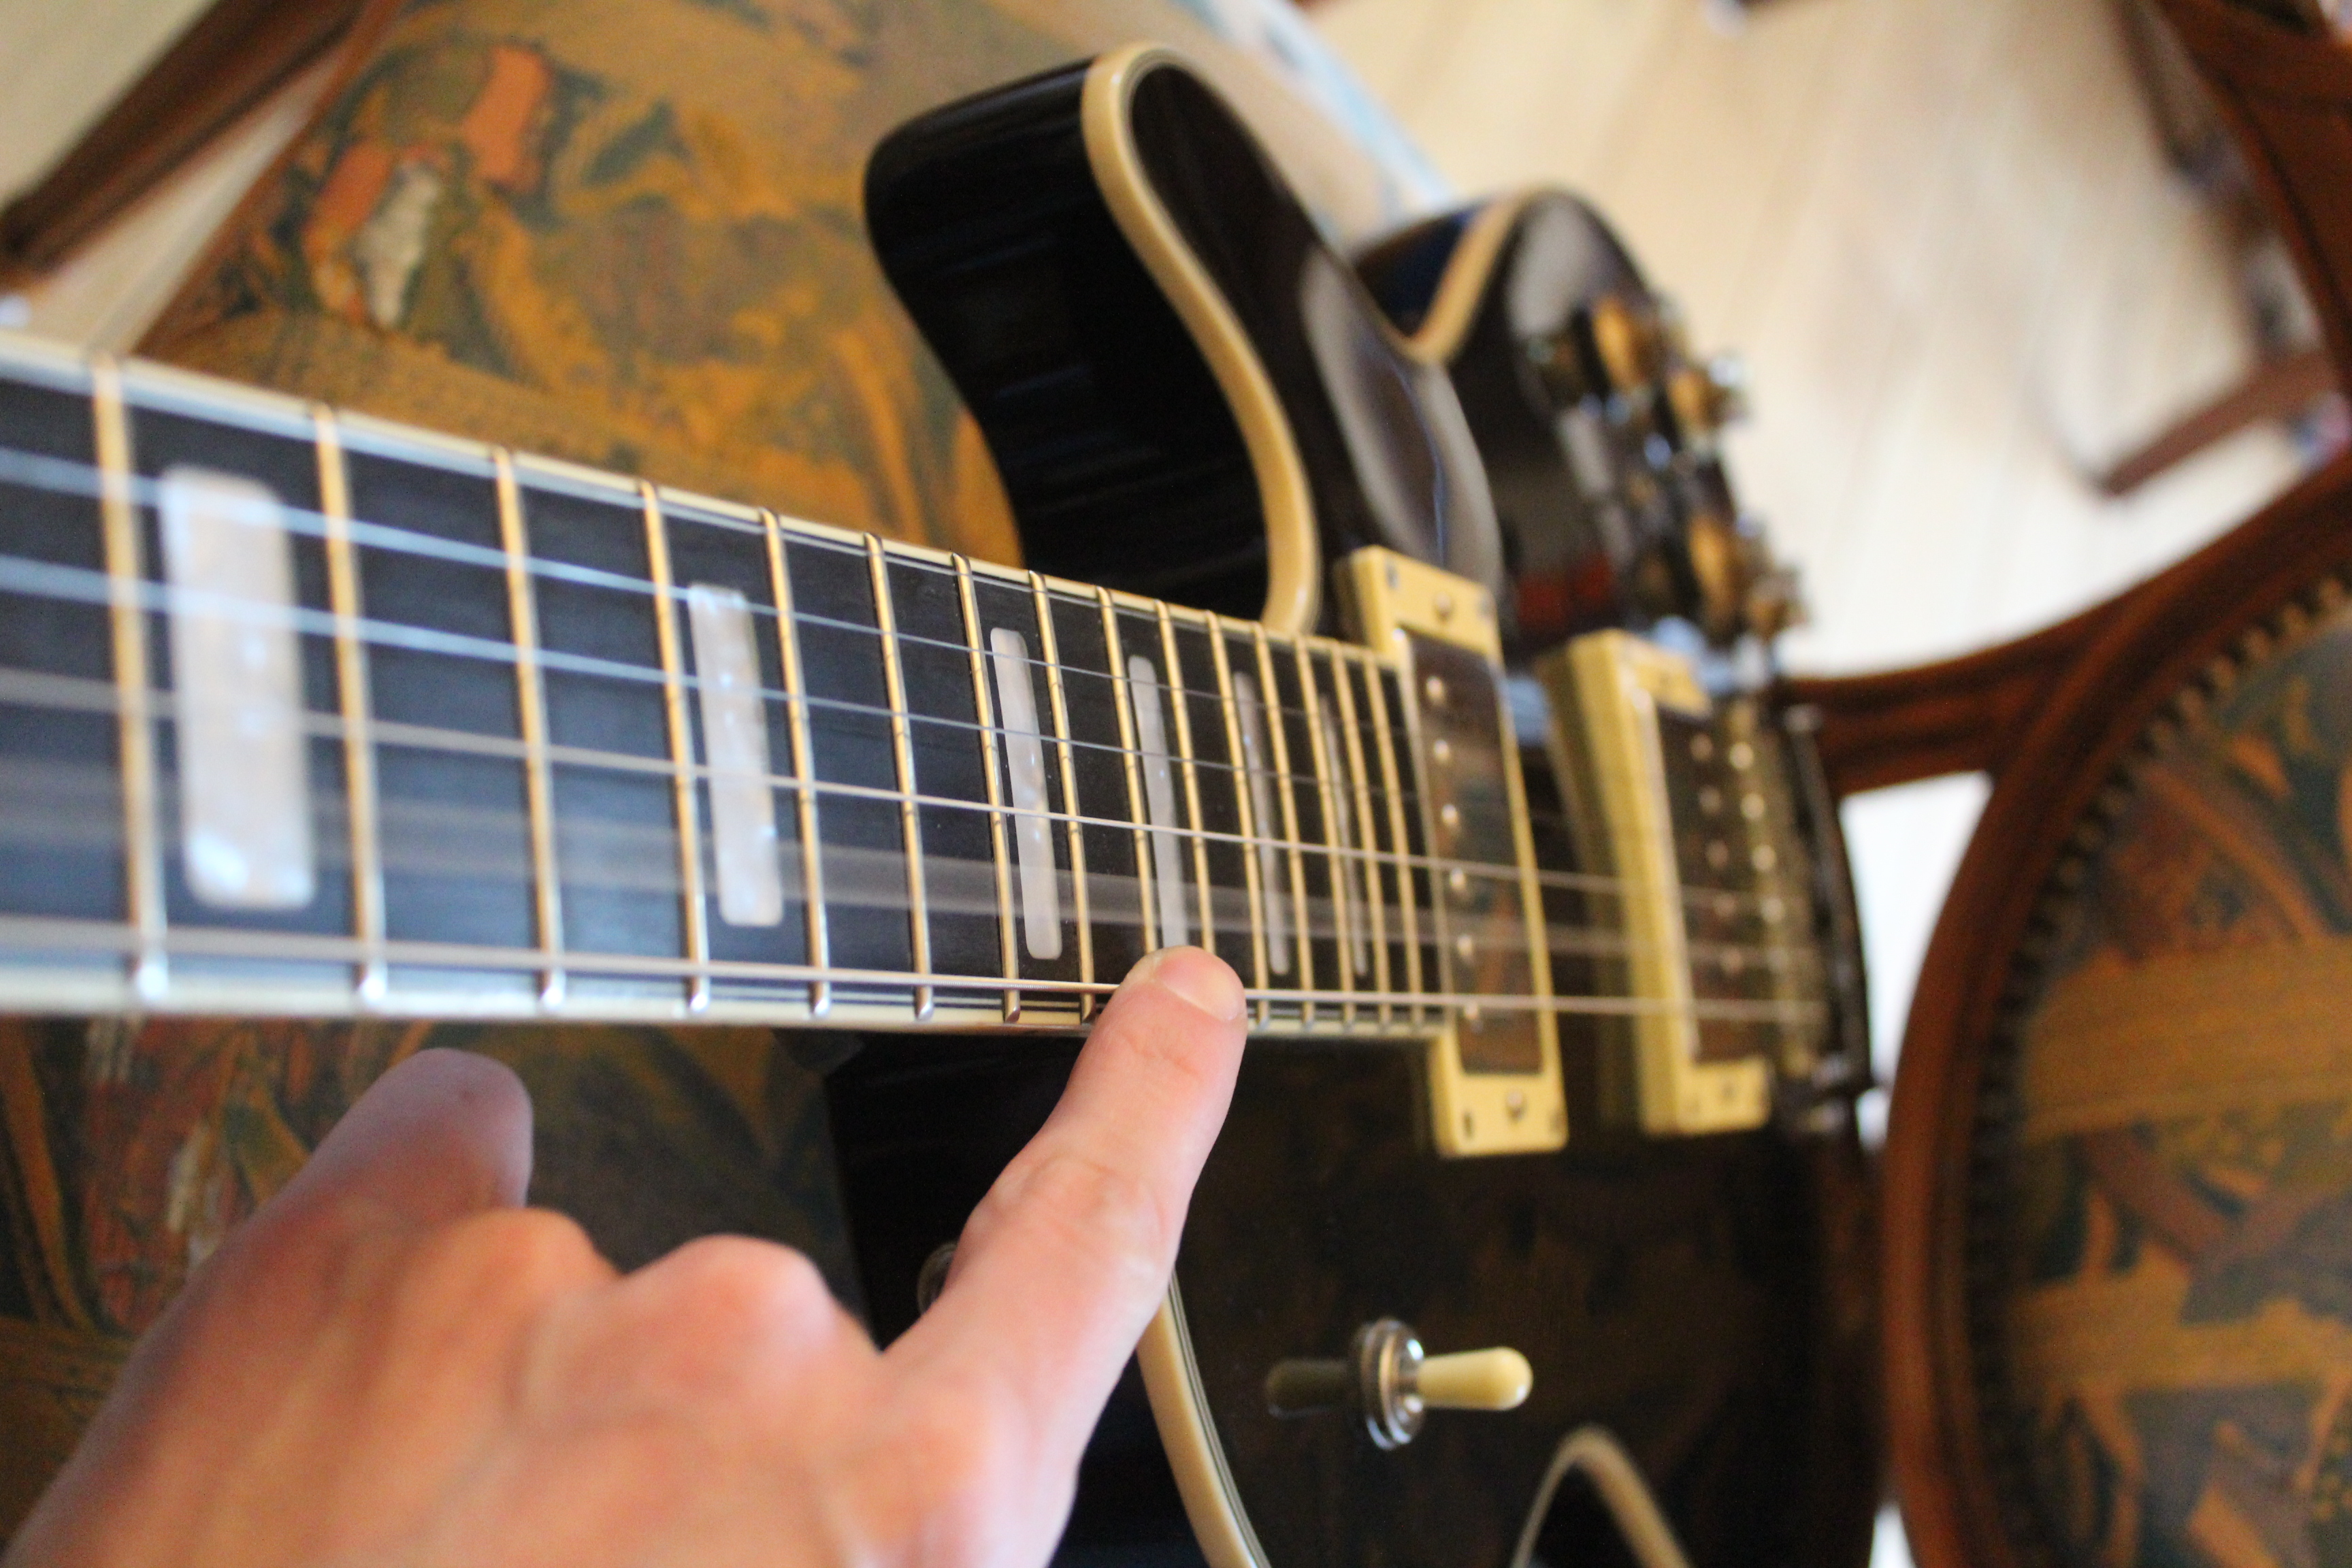
\includegraphics[width=0.9\textwidth]{0Ordnung}
		\caption{Der Grundton auf der zweiten Saite von unten: $A2 \widehat{=} 110Hz$}
		\label{fig:grundton}
\end{figure}

Legt man nun beim Anschlagt einen Finger auf die Saite bei der Hälfte der Länge ohne die Saite herunter zu drücken, erhält man eine stehende Welle mit $k=1$; über dem 12. Bund, wo der Finger die Saite dämpft ist der 3. Knotenpunkt und es gibt 2 Stellen mit konstruktiver Interferenz. (Abbildung \ref{fig:ersteroberton})


Sollte man die Saite \glqq dritteln\grqq , also den Finger über dem 7. Bund (oder 24. Bund) auf die Saite legen, erhält man eine stehende Welle mit $k=2$; es gibt nun insgesamt 4 Knotenpunkte (an Sattel und Brücke, also da, wo die Saite eingespannt ist, unter dem Finger am 7. Bund und am leeren 24. Bund) und 3 konstruktive Interferenzen (Zwischen dem Satten und dem 7. Bund; zwischen dem 7. und 24. Bund; zwischen dem 24. Bund und der Brücke).(Abbildung \ref{fig:zweiteroberton}\endnote{\glqq Stehende Wellen bei Flageoletttönen bei Gitarren\grqq{} von Till Blaha - Eigenes Werk. Lizenziert unter Gemeinfrei.})

\begin{Aufgabe}
Die Mensur einer Gitarre ist an jeder Saite annähernd gleich. Warum ergeben sich trotzdem die unterschiedliche Tonhöhen (Frequenzen) an den einzelnen Saiten, wenn man sie offen spielt (nur anzupft, ohne etwas zu greifen)?

Hinweis 1: Die Mensur, also die Länge der Saite, ist in diesem Fall die Wellenlänge.

Hinweis 2: \gleichungsreferenz{eq:wellen_c}
\end{Aufgabe}

\begin{figure}[!h]
		\centering
		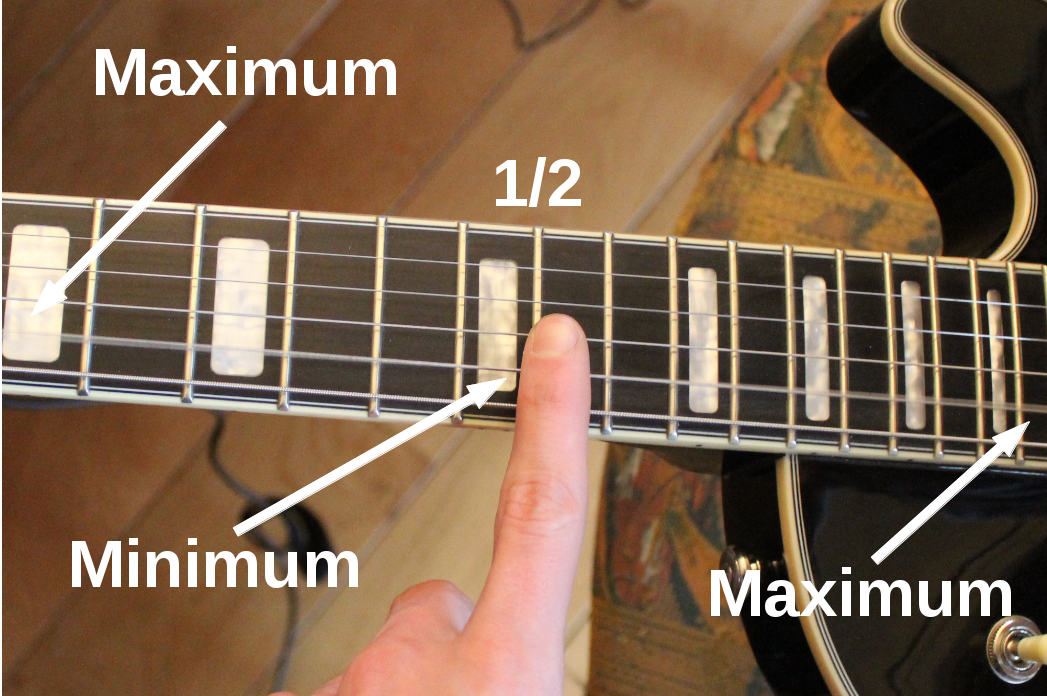
\includegraphics[width=0.8\textwidth]{1Ordnung_Final}
		\caption{Der 1. Oberton auf der zweiten Saite von unten: $A3 \widehat{=} 220Hz$; eine Oktave über dem Grundton}
		\label{fig:ersteroberton}
\end{figure}

\begin{figure}[!h]
		\centering
		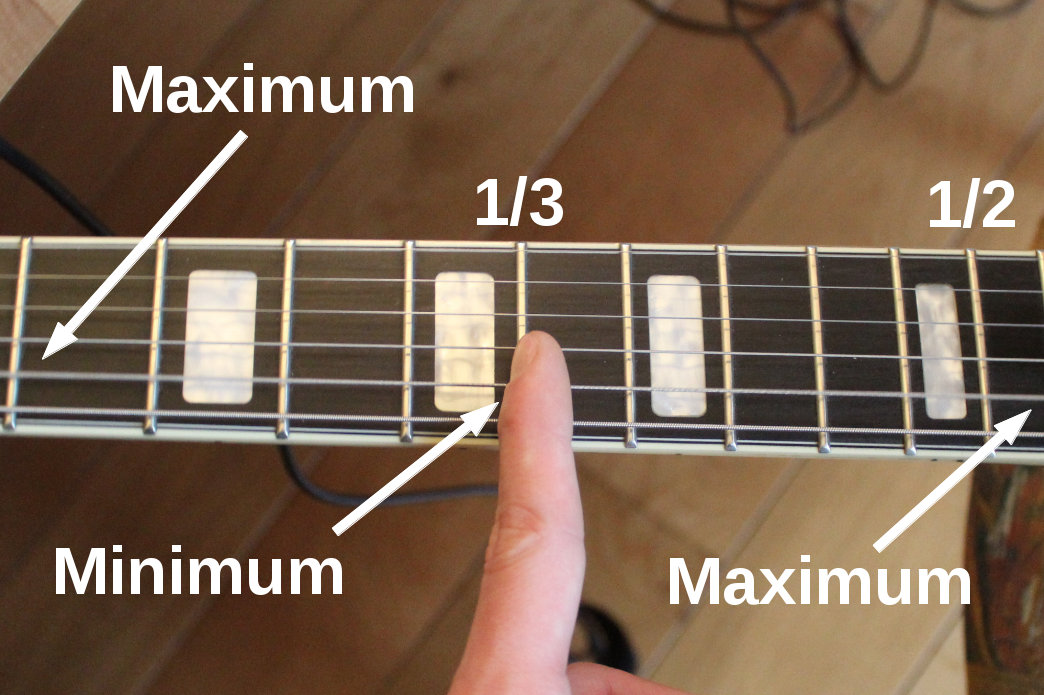
\includegraphics[width=0.8\textwidth]{2Ordnung_Final}
		\caption{Der 2. Oberton auf der zweiten Saite von unten: $E4 \widehat{=} 330Hz$; eine Oktave und eine Quinte über dem Grundton}
		\label{fig:zweiteroberton}
\end{figure}


